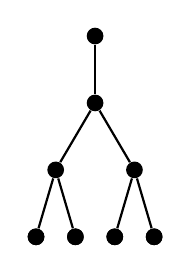
\begin{tikzpicture}[thick,scale=0.5, every node/.style={scale=0.5},level distance=1.7cm]
    \tikzstyle{marrs}=[very thick,-latex]
    \tikzstyle{tnode}=[circle, fill=black, inner sep=1.5mm]
    \tikzstyle{temp}=[inner sep=0mm]
    \def\rstep{5cm}
    
    \huge
    
    \tikzstyle{level 1}=[sibling distance = 4cm];
    \tikzstyle{level 2}=[sibling distance = 2cm];
    \tikzstyle{level 3}=[sibling distance = 1cm];
    
    
    \node[tnode] {}
        child foreach \xi in {1} { node[tnode] {}
            child foreach \yi in {1, 2} { node[tnode] {}
                child foreach \zi in {1, 2} { node[tnode] {}
                    node[tnode] {}
                }
            }
        };
            
\end{tikzpicture}